\section{Cavity with EOM sidebands}
Now, we switched lasers to a 767nm laser and also added an EOM to add sidebands to the laser.
The goal was to measure the linewidth of the cavity peaks more accurately, since we now know that the pizeo is highly unlinear.

In the following, two finesse values will be presented: 
\begin{itemize}
    \item Finesse (distance): This is the ratio between the distance of two adjacent cavity peaks and the FWHM of a peak. Both are measured in ms using the oscilloscpe data. This is similar to just fitting an Airy function
    \item Finesse (500 GHz): Here, the FWHM of a peak is measured using the EOM sideband calibration, thus allowing us to compensate for any piezo hysteresis. The distance is then assumed to be 500 GHz, which should be $\approx \pm 10\%$ of the actual value. This was calculated using $\Delta \nu = \frac{c}{2L}$ with $L\approx300 \mu m$.
\end{itemize}


\begin{figure}[H]
    \centering
    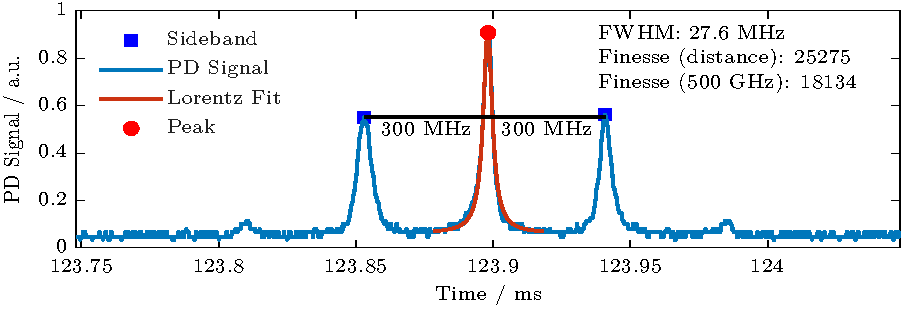
\includegraphics[width=\textwidth]{EOM/Peak2.pdf}
    \caption{Here, the EOM has created two noticable sidebands at a distance of 300 MHz. Knowing this, it was possible to calibrate the time domin to a frequency domain and thus determining the FWHM of the peak. Note that the Finesse is still only given using the non-calibrated time-domain, as we can\'t easily compensate for the non-linearity of the piezo. Also, for this figure, individual Lorentzian peaks have been fitted instead of an entire Airy function. This allowed us to get a kind-of lower and upper-case estimate for the finesse, using both FWHM values for each peak.}
\end{figure}

\begin{figure}[H]
    \centering
    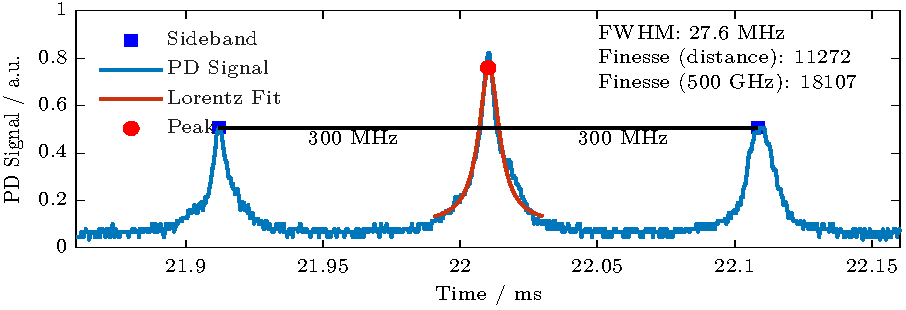
\includegraphics[width=\textwidth]{EOM/Peak1.pdf}
    \caption{Here, the second peak is shown. The x axis scale shows the same time length (0.4 ms) as in the previous figure.}
\end{figure}


Laser issues, worse results possible, calculate over 500 GHz is more reliable

A few things to mention: The laser was not super stable. The above plots are among the best ones that we\'ve been able to capture. For many laser configurations (temperature, power), we saw multimode bevahiour of the cavity.
In some measurements, the calibrated FWHM also differed by up to 30\% between each peak.

Additionally, the difference in the Finesse (distance) and the Finesse (500 GHz) once again shows the non-linear bevahiour of the piezo.
The left peak tends to undererstimate the finesse, whilst the right one tends to overerstimate it. The correct value most likely lies somewhere inbetween.
